\section{Principal Component Analysis \hpoints{30}}

\paragraph{Task description.}
Here we will consider a dataset for optical character recognition (OCR).  
The dataset we provide consists of a sequence of words, one character per row.%
\footnote{This dataset is a modified version of the dataset at
\url{http://www.seas.upenn.edu/~taskar/ocr/}, which has been
subsampled and slightly altered to simplify the processing.}
%
The very first character of each word was capitalized in the original
data and has been omitted for simplicity. The dataset is located in 
{\tt data/ocr\_data.mat}. The format of the data is described in 
{\tt data/data\_format.txt}, so please read that file before continuing.

In this problem you will use PCA to reduce the training data (the 0/1
pixel data of the training set) from 64 dimensions to 20 dimensions. To 
answer the questions you need to write code in Matlab to process
the dataset. {\em You {\bf are} allowed to use built-in matlab function for PCA, K-means, etc. for this problem.}
Note, there is {\em no} automatic grader for this problem
and you do not need to submit your code for grading.

\begin{enumerate}
\item \points{5} Using the top 2 PCA dimensions, display all the test
  letters ``x'' and ``y'', using crosses and circles respectively.
  An example of a plot of ``x'' vs ``w'' is shown in Figure
  \ref{fig:pca_xw} below.

  \begin{figure}[h!]
    \centering
    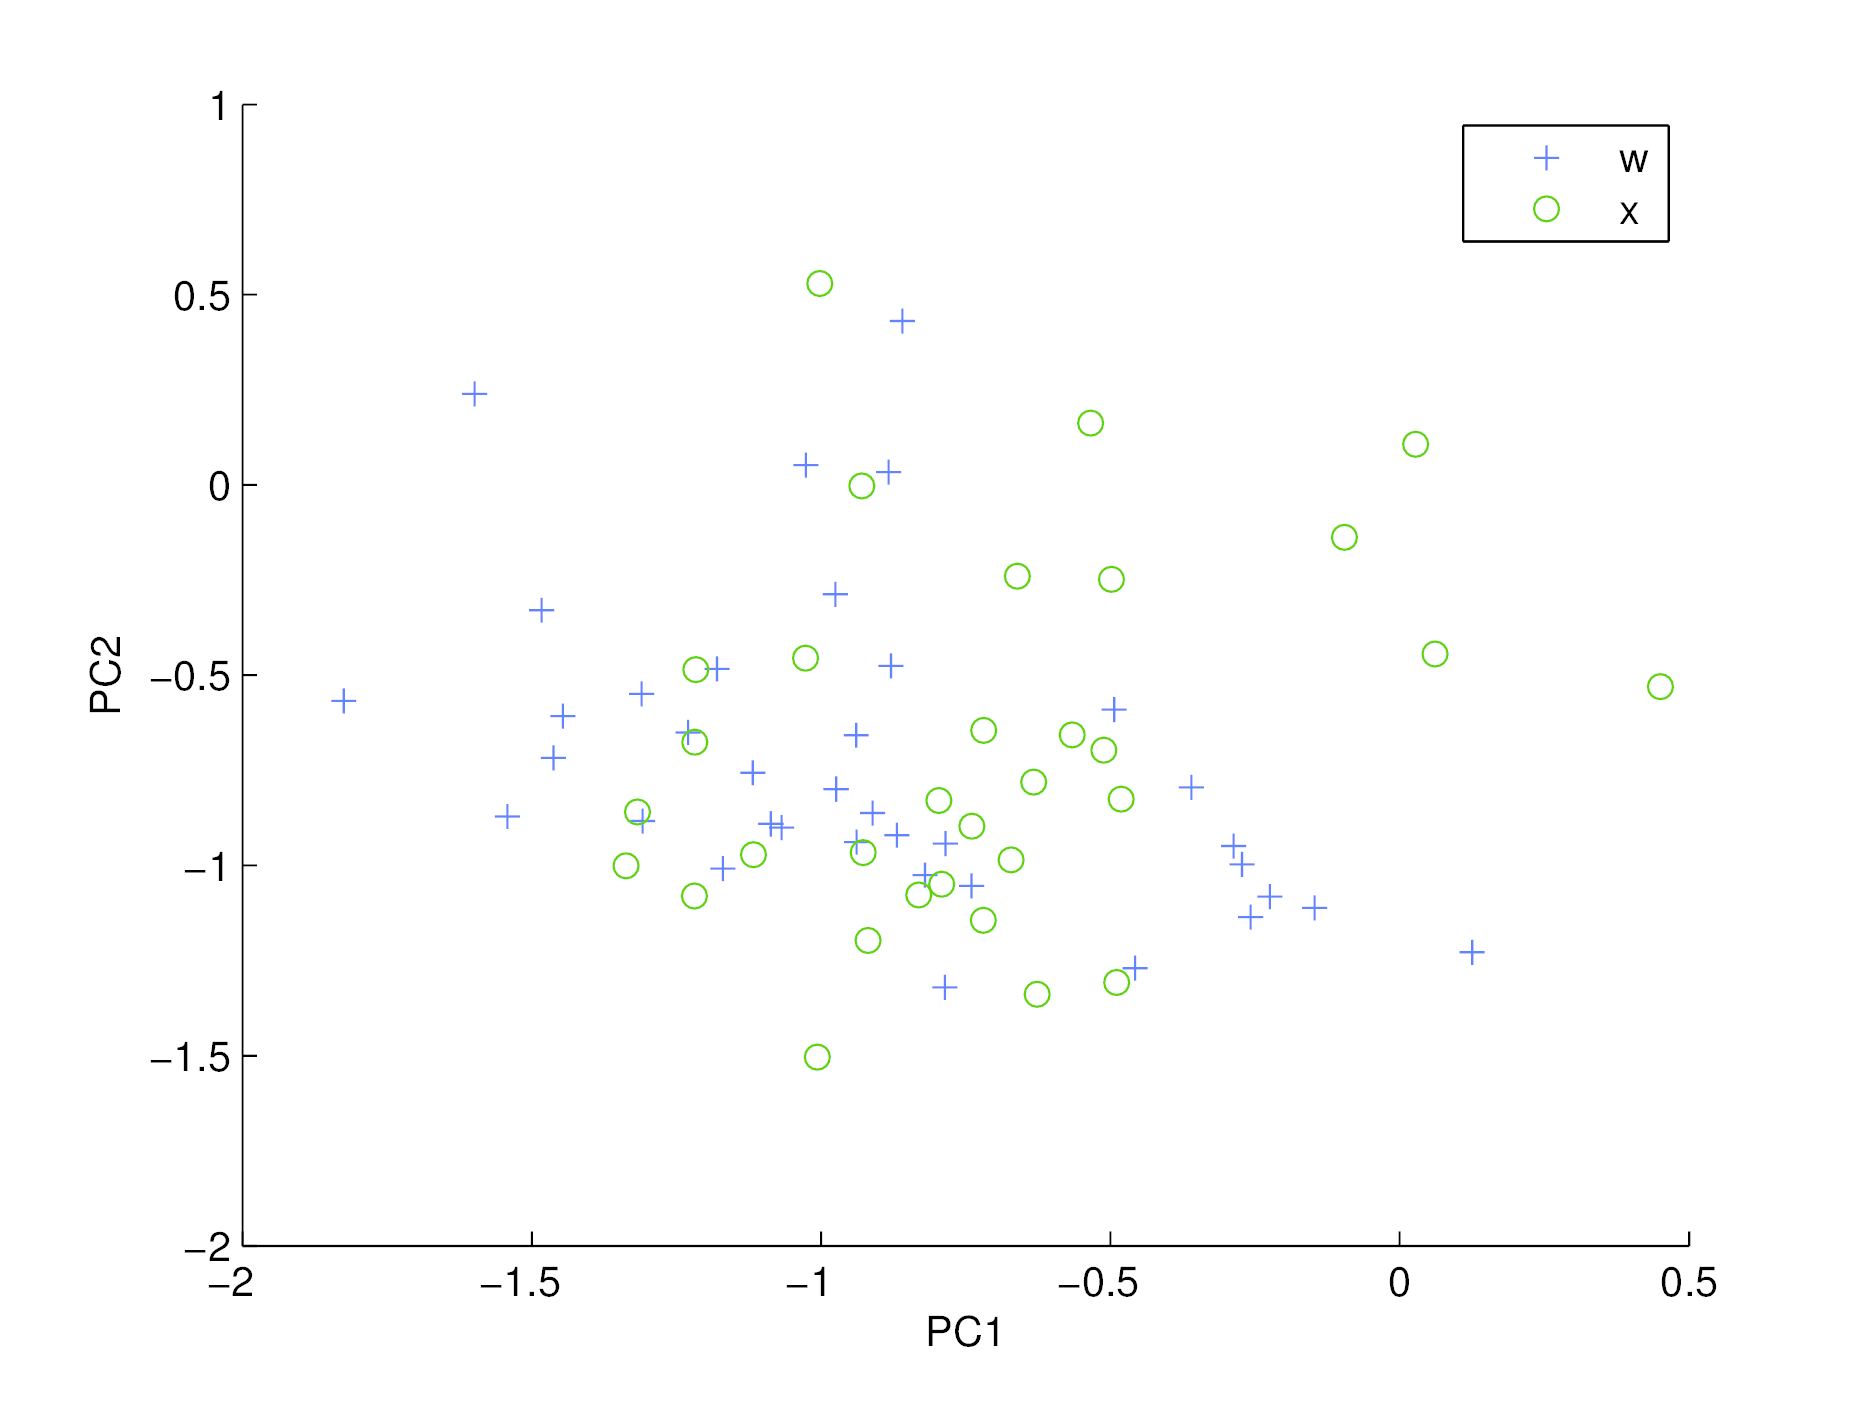
\includegraphics[width=0.65\textwidth]{images/pca_x_w}
    \caption{Plot of 'x'-'w' characters from top 2 PCA
        dimensions}\label{fig:pca_xw}
  \end{figure}

 \begin{figure}[H]
    \centering
    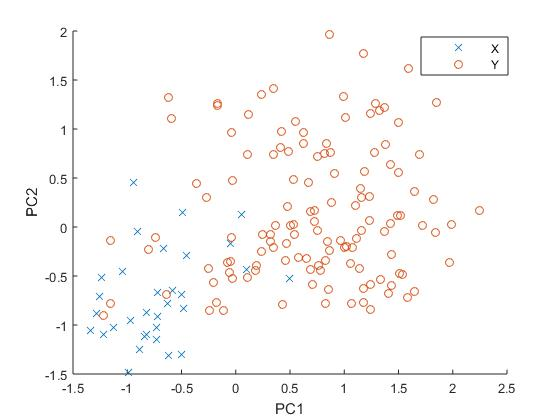
\includegraphics[width=0.65\textwidth]{images/3_1}
    \caption{Plot of 'x'-'y' characters from top 2 PCA
        dimensions}\label{fig:pca_xw}
  \end{figure}
  
\item \points{5} Plot the average (in sample) reconstruction error  $||X - \hat{X}||_F$
of the digits as a function of the number of principle components that are included.  How many
principle components are required to get 90\% reconstruction accuracy? (I.e., to explain 90\% of the 
variance:  $||X - \hat{X}||_F/ ||X - \bar{X}||_F = 0.9$  where $\bar{X}|$ is a matrix, every row of which is the
average $x$ -- the average image.  Reminder: be sure to subtract that mean from $X$ before you find the principle components, 
and to add it back in for your predictions. \\

We get 90% accuracy for 42 dimensions \\


 \begin{figure}[H]
    \centering
    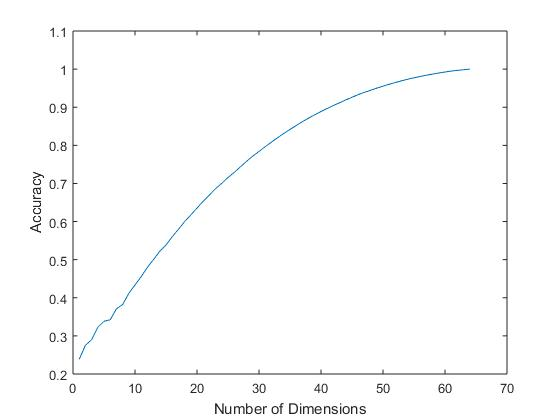
\includegraphics[width=0.65\textwidth]{images/3_2}
    \caption{Error versus number of PCA dimensions
        dimensions}\label{fig:pca_xw}
  \end{figure}



\item \points{10} Learn a Gaussian Naive Bayes classifier using MLE on
  the PCA-ed data and report accuracy on the test set using 5, 10 and
  20 top dimensions.  You should be learning a mean and variance for
  each class and each dimension.  So 26 parameters for class priors,
  and 26 times (5,10 or 20) means plus 26 times (5,10, or 20)
  variances.  In addition to reporting accuracies, write a brief
  description (3-4 sentences) of how these results compare to the
  performance of Naive Bayes on the original data. {\bf Please include your
    source code in your write-up, but do not include built-in matlab functions.} \\

Source Code: \\

\begin{align*}
load('./data/ocr_data.mat');  \\
pooledLetters = [trainset.letter;testset.letter]; \\
pooledPixels = [trainset.pixels;testset.pixels]; \\
[coeff,score,latent] = pca(pooledPixels); \\
pooleddata_5 = score( : , 1:5 ); \\
pooleddata_10 = score(:,1:10); \\
pooleddata_20 = score(:,1:20); \\
trainsize = size(trainset.pixels,1); \\
pooledSize = size(pooledPixels,1); \\
traindata_5 = pooleddata_5(1:trainsize,:); \\
testdata_5 = pooleddata_5(trainsize+1:pooledSize,:); \\
traindata_10 = pooleddata_10(1:trainsize,:); \\
testdata_10 = pooleddata_10(trainsize+1:pooledSize,:); \\
traindata_20 = pooleddata_20(1:trainsize,:); \\
testdata_20 = pooleddata_20(trainsize+1:pooledSize,:); \\
model_5 = fitcnb(traindata_5,trainset.letter); \\
model_10 = fitcnb(traindata_10,trainset.letter); \\
model_20 = fitcnb(traindata_20,trainset.letter); \\
[label_5,Posterior_5,Cost_5] = predict(model_5,testdata_5); \\
[label_10,Posterior_10,Cost_10] = predict(model_10,testdata_10); \\
[label_20,Posterior_20,Cost_20] = predict(model_20,testdata_20); \\
error_5 = find(label_5 ~= testset.letter); \\
error_10 = find(label_10 ~= testset.letter); \\
error_20 = find(label_20 ~= testset.letter); \\
errorval_5 = size(error_5,1)/size(testset.letter,1); \\
errorval_10 = size(error_10,1)/size(testset.letter,1); \\
errorval_20 = size(error_20,1)/size(testset.letter,1); \\
origModel = fitcnb(trainset.pixels,trainset.letter,'Distribution','mvmn'); \\
[label_orig,post_orig,cost_orig] = predict(origModel,testset.pixels); \\
errorOrig = find(label_orig ~= testset.letter); \\
errorValOrig = size(errorOrig,1)/size(testset.letter,1); \\
\end{align*}
The error for Naive Bayes classifier when run on original data is more than when run on the PCA'ed data as we are including only the most important features. \\

Accuracy for Original Data = 0.5434 \\
Accuracy for Naive Bayes with data with 5 dimensions = 0.4366 \\
Accuracy for Naive Bayes with data with 10 dimensions = 0.6013 \\
Accuracy for Naive Bayes with data with 20 dimensions = 0.6630 \\


\item \points{10} Learn a k-means classifier on
  the samePCA-ed data and report accuracy on the test set using 5, 10 and
  20 top dimensions.  In addition to reporting accuracies, write a brief
  description (3-4 sentences) of how these results compare to the
  performance of The Gaussian Naive Bayes classifier. {\bf Please include your 
    source code in your write-up, but do not include built-in matlab functions.} \\

\begin{align*}
 load('./data/ocr_data.mat'); \\
pooledLetters = [trainset.letter;testset.letter]; \\
pooledPixels = [trainset.pixels;testset.pixels]; \\
[coeff,score,latent] = pca(pooledPixels); \\
pooleddata_5 = score(:,1:5); \\
pooleddata_{10} = score(:,1:10); \\
pooleddata_{20} = score(:,1:20); \\
trainsize = size(trainset.pixels,1); \\
pooledSize = size(pooledPixels,1); \\
traindata_5 = pooleddata_5(1:trainsize,:); \\
testdata_5 = pooleddata_5(trainsize+1:pooledSize,:); \\
traindata_{10} =pooleddata_{10}(1:trainsize,:); \\
testdata_{10} = pooleddata_{10}(trainsize+1:pooledSize,:); \\
traindata_{20} =pooleddata_{20}(1:trainsize,:); \\
testdata_{20} =pooleddata_{20}(trainsize+1:pooledSize,:); \\
[idx_5,C_5] = kmeans(traindata_5,153,'MaxIter',300); \\
[idx_{10},C_{10}] = kmeans(traindata_{10},153,'MaxIter',300); \\
[idx_{20},C_{20}] = kmeans(traindata_{20},153,'MaxIter',300); \\
clusterMap_5 = zeros(153,1); \\
clusterMap_{10} = zeros(153,1); \\
clusterMap_{20} = zeros(153,1); \\
for i=1:153 \\
    tempClusterVal = idx_5(:,1) ==i; \\
    vals = trainset.letter(tempClusterVal); \\
    clusterMap_5(i) = mode(vals); \\
    tempClusterVal = idx_{10}(:,1) ==i; \\
    vals = trainset.letter(tempClusterVal); \\
    clusterMap_{10}(i) = mode(vals); \\
    tempClusterVal = find(idx_{20}(:,1) ==i); \\
    vals = trainset.letter(tempClusterVal); \\
    clusterMap_{20}(i) = mode(vals);\\
end\\
closest_5 = zeros(size(testdata_5,1),1); \\
closest_{10} = zeros(size(testdata_{10},1),1); \\
closest_{20} = zeros(size(testdata_{20},1),1); \\
for i=1:size(testdata_5,1) \\
    distances_5 = sqrt(sum(bsxfun(@minus, C_5, testdata_5(i,:)).^2,2)); \\
    closest_5(i) = clusterMap_5(distances_5==min(distances_5)); \\
    distances_10 = sqrt(sum(bsxfun(@minus, C_10, testdata_10(i,:)).^2,2)); \\
    closest_10(i) = clusterMap_10(distances_10==min(distances_10)); \\
    distances_20 = sqrt(sum(bsxfun(@minus, C_20, testdata_20(i,:)).^2,2)); \\
    closest_20(i) = clusterMap_20(distances_20==min(distances_20)); \\
end \\
error_5 = find(closest_5 ~= testset.letter); \\
error_10 = find(closest_10 ~= testset.letter); \\
error_20 = find(closest_20 ~= testset.letter); \\
errorval_5 = size(error_5,1)/size(testset.letter,1); \\
errorval_10 = size(error_10,1)/size(testset.letter,1); \\
errorval_20 = size(error_20,1)/size(testset.letter,1); \\
[idx,C] = kmeans(trainset.pixels,153,'MaxIter',300); \\
closest = zeros(size(testset.pixels,1),1); \\
clusterMap = zeros(153,1); \\
for i=1:153 \\
    tempClusterVal = idx(:,1) ==i; \\
    vals = trainset.letter(tempClusterVal); \\
    clusterMap(i) = mode(vals); \\
end \\
for i=1:size(testset.pixels,1) \\
    distances = sqrt(sum(bsxfun(@minus, C, testset.pixels(i,:)).^2,2)); \\
    closest(i) = clusterMap(distances==min(distances)); \\
end \\
errorOrig = find(closest ~= testset.letter); \\
errorValOrig = size(errorOrig,1)/size(testset.letter,1); \\
\end{align*}

Accuracy for K-Means with 5 clusters = 0.5177 \\
Accuracy for K-Means with 10 clusters =     0.6437 \\
Accuracy for K-Means with 20 clusters =     0.6571 \\
Accuracy for K-Means with original data =     0.6507 \\

Accuracy for K-Means for 20 clusters is better than original \\

\end{enumerate}

